%2multibyte Version: 5.50.0.2960 CodePage: 65001
%TCIDATA{OutputFilter=latex2.dll}
%TCIDATA{Version=5.50.0.2960}
%TCIDATA{Codepage=65001}
%TCIDATA{CSTFile=beamer.cst}
%TCIDATA{Created=Sunday, June 14, 2026 10:00:00}
%TCIDATA{LastRevised=Sunday, June 14, 2026 10:00:00}
%TCIDATA{<META NAME="GraphicsSave" CONTENT="32">}
%TCIDATA{<META NAME="SaveForMode" CONTENT="2">}
%TCIDATA{BibliographyScheme=Manual}
%TCIDATA{<META NAME="DocumentShell" CONTENT="Other Documents\SW\Slides - Beamer">}
%BeginMSIPreambleData
\providecommand{\U}[1]{\protect\rule{.1in}{.1in}}
%EndMSIPreambleData

\documentclass[handout]{beamer}
\usepackage{mathpazo}
\usepackage{multimedia}
\usepackage{amsmath}
\usepackage{amsfonts}
\usepackage{amssymb}
\usepackage{graphicx}
\setcounter{MaxMatrixCols}{30}

\newenvironment{stepenumerate}{\begin{enumerate}[<+->]}{\end{enumerate}}
\newenvironment{stepitemize}{\begin{itemize}[<+->]}{\end{itemize}}
\newenvironment{stepenumeratewithalert}{\begin{enumerate}[<+-| alert@+>]}{\end{enumerate}}
\newenvironment{stepitemizewithalert}{\begin{itemize}[<+-| alert@+>]}{\end{itemize}}
\usetheme{Madrid}

\providecommand{\R}{\mathbb{R}}
\providecommand{\N}{\mathbb{N}}
\providecommand{\E}{\mathbb{E}}
\providecommand{\Prob}{\mathbb{P}}
\providecommand{\Q}{\mathbb{Q}}
\providecommand{\F}{\mathcal{F}}
\providecommand{\B}{\mathcal{B}}
\providecommand{\G}{\mathcal{G}}
\providecommand{\Var}{\operatorname{Var}}
\providecommand{\Cov}{\operatorname{Cov}}
\providecommand{\VaR}{\operatorname{VaR}}
\providecommand{\CVaR}{\operatorname{CVaR}}
\providecommand{\argmin}{\operatorname*{arg\,min}}
\providecommand{\argmax}{\operatorname*{arg\,max}}
\providecommand{\EVPI}{\operatorname{EVPI}}
\providecommand{\VSS}{\operatorname{VSS}}
\providecommand{\QTR}[2]{\csname #1\endcsname{#2}}

\title{Lezione 5 -- Processi stocastici I}
\subtitle{Metodi Quantitativi per la Finanza}
\author[P. Falbo, C. Pelizzari]{{\LARGE Paolo Falbo, Cristian Pelizzari}}
\institute[]{{\large Dipartimento Economia e Management}}
\date[]{}
\titlegraphic{

\includegraphics[width=3.3cm]{../graphics/logo-Unibs-esteso.png}
}

\begin{document}
\maketitle

% ============================================================
% GRUPPO 1 -- APERTURA
% Slide 1-3
% Tempo parziale: 10 minuti | Tempo cumulato: 10 minuti
% ============================================================

\section{Apertura}

% --------------------------------------------------------
% Slide 1 -- Domanda guida
% --------------------------------------------------------

\subsection{Domanda guida}

%TCIMACRO{\TeXButton{BeginFrame}{\begin{frame}}}%
%BeginExpansion
\begin{frame}%
%EndExpansion

\QTR{frametitle}{Lezione 5 -- Processi stocastici I}

%TCIMACRO{\TeXButton{Transparency}{\setbeamercovered{transparent=20}}}%
%BeginExpansion
\setbeamercovered{transparent=20}%
%EndExpansion

\begin{center}
{\Large Come si rappresenta l'evoluzione temporale\\
dell'incertezza quando l'informazione cresce nel tempo?}
\end{center}

\medskip

In finanza molte grandezze non sono statiche, ma evolvono nel tempo:

\begin{stepitemize}
\item il prezzo di un'azione giorno per giorno;
\item il merito creditizio di una controparte nel corso degli anni;
\item il tasso di inflazione lungo un orizzonte pluriennale;
\item il valore di un portafoglio sotto scenari futuri alternativi.
\end{stepitemize}

\medskip

Una singola variabile casuale non basta. Serve un oggetto che evolve:
\[
\{X_t\}_{t=0}^{T}.
\]

%TCIMACRO{\TeXButton{Transition: Box Out}{\transboxout}}%
%BeginExpansion
\transboxout
%EndExpansion
%TCIMACRO{\TeXButton{EndFrame}{\end{frame}}}%
%BeginExpansion
\end{frame}%
%EndExpansion

% --------------------------------------------------------
% Slide 2 -- Percorso della lezione
% --------------------------------------------------------

\subsection{Percorso della lezione}

%TCIMACRO{\TeXButton{BeginFrame}{\begin{frame}}}%
%BeginExpansion
\begin{frame}%
%EndExpansion

\QTR{frametitle}{Percorso della lezione}

%TCIMACRO{\TeXButton{Transparency}{\setbeamercovered{transparent=20}}}%
%BeginExpansion
\setbeamercovered{transparent=20}%
%EndExpansion

L'obiettivo \`{e} costruire il linguaggio dei processi stocastici
in tempo discreto e applicarlo a un primo modello concreto.

\medskip

\begin{stepenumerate}
\item[1.] Processo stocastico: definizione e traiettorie.
\item[2.] Momenti e dipendenza temporale: $\mu(t)$, $\sigma^2(t)$, $c(s,t)$.
\item[3.] Filtrazione e adattabilit\`{a}: informazione che cresce nel tempo.
\item[4.] Martingale: il concetto di gioco equo e le sue implicazioni.
\item[5.] Il modello binomiale come palestra strutturale.
\item[6.] Esercizi in aula e sintesi.
\end{stepenumerate}

\medskip

\begin{center}
{\small Tutti gli strumenti di questa lezione valgono per qualunque
processo, discreto o continuo.}
\end{center}

%TCIMACRO{\TeXButton{Transition: Box Out}{\transboxout}}%
%BeginExpansion
\transboxout
%EndExpansion
%TCIMACRO{\TeXButton{EndFrame}{\end{frame}}}%
%BeginExpansion
\end{frame}%
%EndExpansion

% ============================================================
% Slides_Lez_05_Gruppo_02_Processo.tex
% GRUPPO 2 -- Processo stocastico: definizione e traiettorie
% Slide 4-7
% Tempo parziale: 15 minuti | Tempo cumulato: 25 minuti
% ============================================================

\section{Processo stocastico}

% --------------------------------------------------------
% Slide 4 -- Definizione
% --------------------------------------------------------

\subsection{Definizione}

%TCIMACRO{\TeXButton{BeginFrame}{\begin{frame}}}%
%BeginExpansion
\begin{frame}%
%EndExpansion

\QTR{frametitle}{Processo stocastico: definizione}

%TCIMACRO{\TeXButton{Transparency}{\setbeamercovered{transparent=20}}}%
%BeginExpansion
\setbeamercovered{transparent=20}%
%EndExpansion

Un \textbf{processo stocastico} \`{e} una famiglia di variabili casuali
indicizzata dal tempo:
\[
\{X_t\}_{t \in \mathcal{T}}, \qquad X_t : \Omega \rightarrow \mathbb{R}.
\]

\medskip

\begin{stepitemize}
\item L'insieme degli indici $\mathcal{T}$ pu\`{o} essere discreto
($\mathcal{T} = \{0,1,\ldots,T\}$) o continuo ($\mathcal{T} = [0,T]$).
\item Per ogni istante $t$ fissato, $X_t$ \`{e} una variabile casuale:
descrive l'incertezza sul valore del processo a quell'istante.
\item Per ogni esito $\omega \in \Omega$ fissato, $t \mapsto X_t(\omega)$
\`{e} una funzione deterministica del tempo: la \textbf{traiettoria}.
\end{stepitemize}


%TCIMACRO{\TeXButton{Transition: Box Out}{\transboxout}}%
%BeginExpansion
\transboxout
%EndExpansion
%TCIMACRO{\TeXButton{EndFrame}{\end{frame}}}%
%BeginExpansion
\end{frame}%
%EndExpansion

% --------------------------------------------------------
% Slide 5 -- Tre livelli di lettura
% --------------------------------------------------------

\subsection{Tre livelli di lettura}

%TCIMACRO{\TeXButton{BeginFrame}{\begin{frame}}}%
%BeginExpansion
\begin{frame}%
%EndExpansion

\QTR{frametitle}{Tre livelli di lettura}

%TCIMACRO{\TeXButton{Transparency}{\setbeamercovered{transparent=20}}}%
%BeginExpansion
\setbeamercovered{transparent=20}%
%EndExpansion

Lo stesso oggetto $\{X_t\}$ si pu\`{o} leggere in tre modi:

\medskip

\begin{stepitemize}

\item \textbf{Distribuzione marginale} -- fissato $t$, $X_t$ \`{e} una
variabile casuale con la sua distribuzione:
\[
\Prob(X_t \leq x), \quad \E[X_t], \quad \Var(X_t).
\]
Descrive l'incertezza sul valore a un istante dato.

\item \textbf{Traiettoria} -- fissato $\omega$, la mappa
$t \mapsto X_t(\omega)$ \`{e} una sequenza di numeri:
\[
X_0(\omega),\; X_1(\omega),\; \ldots,\; X_T(\omega).
\]
\`{E} il percorso realizzato in uno specifico scenario.

\item \textbf{Famiglia} -- l'intero oggetto $\{X_t\}_{t=0}^T$ descrive
la struttura congiunta: come i valori ai diversi istanti si
influenzano e si correlano.

\end{stepitemize}

%TCIMACRO{\TeXButton{Transition: Box Out}{\transboxout}}%
%BeginExpansion
\transboxout
%EndExpansion
%TCIMACRO{\TeXButton{EndFrame}{\end{frame}}}%
%BeginExpansion
\end{frame}%
%EndExpansion

% --------------------------------------------------------
% Slide 6 -- Esempio finanziario: prezzo su più periodi
% --------------------------------------------------------

\subsection{Esempio finanziario}

%TCIMACRO{\TeXButton{BeginFrame}{\begin{frame}}}%
%BeginExpansion
\begin{frame}%
%EndExpansion

\QTR{frametitle}{(*) Esempio: il prezzo di un'azione su pi\`{u} periodi}

%TCIMACRO{\TeXButton{Transparency}{\setbeamercovered{transparent=20}}}%
%BeginExpansion
\setbeamercovered{transparent=20}%
%EndExpansion

Sia $S_t$ il prezzo di un'azione al tempo $t = 0, 1, 2, 3$.

\medskip

\begin{stepitemize}

\item \textbf{Distribuzione marginale}: al tempo $t=2$ il prezzo $S_2$
\`{e} una variabile casuale. Possiamo chiederci: qual \`{e} il suo
valore atteso? Qual \`{e} la sua varianza?

\item \textbf{Traiettoria}: in uno scenario $\omega$ specifico, il
prezzo percorre un cammino:
\[
S_0(\omega) = 100,\quad S_1(\omega) = 110,\quad
S_2(\omega) = 99,\quad S_3(\omega) = 108.9.
\]
Ogni scenario corrisponde a una diversa sequenza di rialzi e ribassi.

\item \textbf{Famiglia}: la struttura congiunta di $S_0, S_1, S_2, S_3$
risponde a domande come: il prezzo di oggi \`{e} correlato con quello
di dopodomani? Come evolve l'incertezza sul prezzo al crescere
dell'orizzonte?

\end{stepitemize}

%TCIMACRO{\TeXButton{Transition: Box Out}{\transboxout}}%
%BeginExpansion
\transboxout
%EndExpansion
%TCIMACRO{\TeXButton{EndFrame}{\end{frame}}}%
%BeginExpansion
\end{frame}%
%EndExpansion

% --------------------------------------------------------
% Slide 7 -- Spazio campionario e traiettorie
% --------------------------------------------------------

\subsection{Spazio campionario e traiettorie}

%TCIMACRO{\TeXButton{BeginFrame}{\begin{frame}}}%
%BeginExpansion
\begin{frame}%
%EndExpansion

\QTR{frametitle}{Spazio campionario e traiettorie}

%TCIMACRO{\TeXButton{Transparency}{\setbeamercovered{transparent=20}}}%
%BeginExpansion
\setbeamercovered{transparent=20}%
%EndExpansion

Il processo $\{X_t\}$ vive sullo stesso spazio di probabilit\`{a}
$(\Omega, \mathcal{F}, \Prob)$ delle variabili casuali delle lezioni
precedenti.

\medskip

\begin{stepitemize}

\item Ogni esito elementare $\omega \in \Omega$ seleziona
\textbf{un'intera traiettoria}: non un singolo numero, ma una
sequenza $X_0(\omega), X_1(\omega), \ldots, X_T(\omega)$.

\item L'insieme di tutte le traiettorie possibili forma lo
\textbf{spazio delle traiettorie}: ogni $\omega$ corrisponde a
un percorso diverso.

\item La probabilit\`{a} $\Prob$ assegna un peso a ogni traiettoria
(o a insiemi di traiettorie): i percorsi pi\`{u} probabili hanno
peso maggiore.

\item Un processo a tempo discreto con $T$ periodi e stati finiti
ha un numero finito di traiettorie. Nel modello binomiale con
$T$ periodi: $2^T$ traiettorie.

\end{stepitemize}

%TCIMACRO{\TeXButton{Transition: Box Out}{\transboxout}}%
%BeginExpansion
\transboxout
%EndExpansion
%TCIMACRO{\TeXButton{EndFrame}{\end{frame}}}%
%BeginExpansion
\end{frame}%
%EndExpansion

% ============================================================
% Slides_Lez_05_Gruppo_03_Momenti.tex
% GRUPPO 3 -- Momenti e dipendenza temporale
% Slide 8-12
% Tempo parziale: 15 minuti | Tempo cumulato: 40 minuti
% ============================================================

\section{Momenti e dipendenza temporale}

% --------------------------------------------------------
% Slide 8 -- Le tre funzioni caratteristiche
% --------------------------------------------------------

\subsection{Le tre funzioni caratteristiche}

%TCIMACRO{\TeXButton{BeginFrame}{\begin{frame}}}%
%BeginExpansion
\begin{frame}%
%EndExpansion

\QTR{frametitle}{Le tre funzioni caratteristiche}

%TCIMACRO{\TeXButton{Transparency}{\setbeamercovered{transparent=20}}}%
%BeginExpansion
\setbeamercovered{transparent=20}%
%EndExpansion

Per descrivere un processo senza specificarne l'intera legge,
si usano tre funzioni del tempo:

\medskip

\begin{stepitemize}

\item \textbf{Funzione media}
\[
\mu(t) = \E[X_t].
\]
Livello medio del processo all'istante $t$.

\item \textbf{Funzione varianza}
\[
\sigma^2(t) = \Var(X_t).
\]
Dispersione attorno alla media all'istante $t$: misura l'incertezza
sul valore del processo in quell'istante.

\item \textbf{Funzione di autocovarianza}
\[
c(s,t) = \Cov(X_s, X_t), \qquad s,t \in \mathcal{T}.
\]
Dipendenza lineare tra i valori del processo a due istanti diversi.

\end{stepitemize}

\medskip

\begin{center}
{\small Nota: $c(t,t) = \Var(X_t) = \sigma^2(t)$.}
\end{center}

%TCIMACRO{\TeXButton{Transition: Box Out}{\transboxout}}%
%BeginExpansion
\transboxout
%EndExpansion
%TCIMACRO{\TeXButton{EndFrame}{\end{frame}}}%
%BeginExpansion
\end{frame}%
%EndExpansion

% --------------------------------------------------------
% Slide 9 -- Significato finanziario
% --------------------------------------------------------

\subsection{Significato finanziario}

%TCIMACRO{\TeXButton{BeginFrame}{\begin{frame}}}%
%BeginExpansion
\begin{frame}%
%EndExpansion

\QTR{frametitle}{(*) Significato finanziario}

%TCIMACRO{\TeXButton{Transparency}{\setbeamercovered{transparent=20}}}%
%BeginExpansion
\setbeamercovered{transparent=20}%
%EndExpansion

Le tre funzioni rispondono a domande operative concrete.

\medskip

\begin{stepitemize}

\item $\mu(t)$: \textbf{qual \`{e} il valore atteso del prezzo
(o del tasso) al tempo $t$?}\\
Utile per stimare il rendimento atteso su un orizzonte.

\item $\sigma^2(t)$: \textbf{quanto \`{e} incerto il valore
all'orizzonte $t$?}\\
L'incertezza tipicamente cresce con $t$: il futuro lontano
\`{e} pi\`{u} difficile da prevedere del futuro prossimo.

\item $c(s,t)$: \textbf{il valore di oggi \`{e} correlato
con il valore di domani?}\\
Se $c(s,t) > 0$: un valore elevato oggi tende ad
accompagnarsi a un valore elevato in futuro.\\
Se $c(s,t) = 0$: i valori ai due istanti sono incorrelati --
il passato non aiuta a prevedere il futuro.

\end{stepitemize}

%TCIMACRO{\TeXButton{Transition: Box Out}{\transboxout}}%
%BeginExpansion
\transboxout
%EndExpansion
%TCIMACRO{\TeXButton{EndFrame}{\end{frame}}}%
%BeginExpansion
\end{frame}%
%EndExpansion

% --------------------------------------------------------
% Slide 10 -- Esempio 1: rumore i.i.d.
% --------------------------------------------------------

\subsection{Esempi}
 
%TCIMACRO{\TeXButton{BeginFrame}{\begin{frame}}}%
%BeginExpansion
\begin{frame}%
%EndExpansion
 
\QTR{frametitle}{Esempio 1: rendimenti giornalieri i.i.d.}
 
%TCIMACRO{\TeXButton{Transparency}{\setbeamercovered{transparent=20}}}%
%BeginExpansion
\setbeamercovered{transparent=20}%
%EndExpansion
 
Sia $X_t$ il \textbf{rendimento percentuale} di un'azione
nel giorno $t$. Sotto l'ipotesi di mercato efficiente i
rendimenti giornalieri sono i.i.d.:
$\E[X_t] = \nu$, $\Var(X_t) = \tau^2$ uguali per ogni $t$.
 
\medskip
 
\begin{stepitemize}
 
\item \textbf{Media costante:}
\[
\mu(t) = \E[X_t] = \nu \quad \text{per ogni } t.
\]
Il rendimento atteso non dipende dal giorno.
 
\item \textbf{Varianza costante:}
\[
\sigma^2(t) = \Var(X_t) = \tau^2 \quad \text{per ogni } t.
\]
Il rischio giornaliero non cambia nel tempo.
 
\item \textbf{Covarianza nulla:}
\[
c(s,t) = \Cov(X_s, X_t) = 0 \quad \text{per ogni } s \neq t.
\]
Il rendimento di ieri non aiuta a prevedere quello di oggi:
\textbf{ipotesi di mercato efficiente in forma debole}.
 
\end{stepitemize}
 
%TCIMACRO{\TeXButton{Transition: Box Out}{\transboxout}}%
%BeginExpansion
\transboxout
%EndExpansion
%TCIMACRO{\TeXButton{EndFrame}{\end{frame}}}%
%BeginExpansion
\end{frame}%
%EndExpansion

% --------------------------------------------------------
% Slide 11 -- Esempio 2: passeggiata aleatoria
% --------------------------------------------------------

%TCIMACRO{\TeXButton{BeginFrame}{\begin{frame}}}%
%BeginExpansion
\begin{frame}%
%EndExpansion

\QTR{frametitle}{Esempio 2: passeggiata aleatoria}

%TCIMACRO{\TeXButton{Transparency}{\setbeamercovered{transparent=20}}}%
%BeginExpansion
\setbeamercovered{transparent=20}%
%EndExpansion

Sia $X_0 = 0$ e $X_t = Z_1 + Z_2 + \cdots + Z_t$, ove $Z_k$ sono v.c. i.i.d. con $\E[Z_k] = \nu$, $\Var(Z_k) = \tau^2$ costanti. Il processo $X_t$ si chiama \textbf{passeggiata aleatoria} e risulta:

\medskip

\begin{stepitemize}

\item \textbf{Media dipendente da $\nu$:}
\[
\mu(t) = t\,\nu.
\]

\item \textbf{Varianza crescente:}
\[
\sigma^2(t) = t\,\tau^2.
\]
L'incertezza si \textbf{accumula} nel tempo: l'orizzonte
lontano \`{e} pi\`{u} incerto di quello vicino.

\item \textbf{Covarianza:} per $s \leq t$,
\[
c(s,t) = \min(s,t)\,\tau^2 = s\,\tau^2.
\]
I valori a istanti diversi sono \textbf{correlati positivamente}:
traiettorie che partono alte tendono a restare alte e viceversa.

\end{stepitemize}

%TCIMACRO{\TeXButton{Transition: Box Out}{\transboxout}}%
%BeginExpansion
\transboxout
%EndExpansion
%TCIMACRO{\TeXButton{EndFrame}{\end{frame}}}%
%BeginExpansion
\end{frame}%
%EndExpansion

% --------------------------------------------------------
% Slide 12 -- Confronto e ponte al moto browniano
% --------------------------------------------------------

%TCIMACRO{\TeXButton{BeginFrame}{\begin{frame}}}%
%BeginExpansion
\begin{frame}%
%EndExpansion

\QTR{frametitle}{(*) Confronto e ponte al tempo continuo (Lezione 6)}

%TCIMACRO{\TeXButton{Transparency}{\setbeamercovered{transparent=20}}}%
%BeginExpansion
\setbeamercovered{transparent=20}%
%EndExpansion

\begin{center}
\begin{tabular}{lcc}
\hline
& \textbf{Rendimenti i.i.d.} & \textbf{Passeggiata aleatoria}\\
\hline
$\mu(t)$ & $\nu$ (costante) & $t\,\nu$ (crescente)\\
$\sigma^2(t)$ & $\tau^2$ (costante) & $t\,\tau^2$ (crescente)\\
$c(s,t)$ & $0$ & $\min(s,t)\,\tau^2$\\
Struttura temporale & nessuna & accumulo nel tempo\\
\hline
\end{tabular}
\end{center}

\medskip

\begin{stepitemize}

\item La varianza $\sigma^2(t) = t\,\tau^2$ della passeggiata aleatoria
cresce \textbf{linearmente} con il tempo: raddoppiare l'orizzonte
raddoppia l'incertezza sul valore finale.

\item La struttura di covarianza $c(s,t) = \min(s,t)\,\tau^2$
ricompare \textbf{identica} nel moto browniano standard (Lezione 6),
di cui la passeggiata aleatoria \`{e} l'analogo discreto.

\end{stepitemize}

%TCIMACRO{\TeXButton{Transition: Box Out}{\transboxout}}%
%BeginExpansion
\transboxout
%EndExpansion
%TCIMACRO{\TeXButton{EndFrame}{\end{frame}}}%
%BeginExpansion
\end{frame}%
%EndExpansion

% ============================================================
% Slides_Lez_05_Gruppo_04_Filtrazione.tex
% GRUPPO 4 -- Filtrazione e adattabilità
% Slide 13-18
% Tempo parziale: 20 minuti | Tempo cumulato: 60 minuti
% ============================================================

\section{Filtrazione e adattabilit\`{a}}

% --------------------------------------------------------
% Slide 13 -- Il problema: informazione che cresce nel tempo
% --------------------------------------------------------

\subsection{Informazione che cresce nel tempo}

%TCIMACRO{\TeXButton{BeginFrame}{\begin{frame}}}%
%BeginExpansion
\begin{frame}%
%EndExpansion

\QTR{frametitle}{Il problema: informazione che cresce nel tempo}

%TCIMACRO{\TeXButton{Transparency}{\setbeamercovered{transparent=20}}}%
%BeginExpansion
\setbeamercovered{transparent=20}%
%EndExpansion

Nei capitoli precedenti l'informazione era rappresentata da
una sigma-algebra $\mathcal{G} \subseteq \mathcal{F}$
(Lezione 3).

\medskip

\begin{stepitemize}

\item In un processo stocastico l'informazione non \`{e} statica:
\textbf{cresce nel tempo} man mano che si osservano i valori
del processo.

\item Al tempo $t=0$ non si sa ancora nulla (o quasi).
Al tempo $t=1$ si conosce $X_1$. Al tempo $t=2$ si conoscono
$X_1$ e $X_2$. E cos\`{\i} via.

\item La struttura naturale non \`{e} una singola sigma-algebra,
ma una \textbf{famiglia crescente} di sigma-algebre: una per
ogni istante.

\item In finanza questo corrisponde al flusso di informazioni
di mercato: prezzi, tassi, indici che arrivano progressivamente.

\end{stepitemize}

%TCIMACRO{\TeXButton{Transition: Box Out}{\transboxout}}%
%BeginExpansion
\transboxout
%EndExpansion
%TCIMACRO{\TeXButton{EndFrame}{\end{frame}}}%
%BeginExpansion
\end{frame}%
%EndExpansion

% --------------------------------------------------------
% Slide 14 -- Definizione di filtrazione
% --------------------------------------------------------

\subsection{Filtrazione}

%TCIMACRO{\TeXButton{BeginFrame}{\begin{frame}}}%
%BeginExpansion
\begin{frame}%
%EndExpansion

\QTR{frametitle}{Filtrazione}

%TCIMACRO{\TeXButton{Transparency}{\setbeamercovered{transparent=20}}}%
%BeginExpansion
\setbeamercovered{transparent=20}%
%EndExpansion

\begin{block}{Definizione}
Una \textbf{filtrazione} \`{e} una famiglia di sigma-algebre
$\{\mathcal{F}_t\}_{t=0}^T$ tale che
\[
\mathcal{F}_0 \subseteq \mathcal{F}_1 \subseteq \cdots
\subseteq \mathcal{F}_T \subseteq \mathcal{F}.
\]
\end{block}

\medskip

\begin{stepitemize}

\item La condizione di \textbf{crescita} $\mathcal{F}_s \subseteq
\mathcal{F}_t$ per $s \leq t$ esprime che l'informazione non
diminuisce mai: ci\`{o} che \`{e} noto al tempo $s$ resta noto
a ogni istante successivo.

\item $\mathcal{F}_0$: informazione iniziale -- tipicamente
banale, $\{\emptyset, \Omega\}$: nulla \`{e} ancora osservato.

\item $\mathcal{F}_T$: informazione finale -- tutta la storia
del processo \`{e} nota.

\item Ogni $\mathcal{F}_t$ rappresenta ci\`{o} che un osservatore
sa al tempo $t$ avendo seguito il processo fino a quell'istante.

\end{stepitemize}

%TCIMACRO{\TeXButton{Transition: Box Out}{\transboxout}}%
%BeginExpansion
\transboxout
%EndExpansion
%TCIMACRO{\TeXButton{EndFrame}{\end{frame}}}%
%BeginExpansion
\end{frame}%
%EndExpansion

% --------------------------------------------------------
% Slide 15 -- Filtrazione naturale
% --------------------------------------------------------

\subsection{Filtrazione naturale}

%TCIMACRO{\TeXButton{BeginFrame}{\begin{frame}}}%
%BeginExpansion
\begin{frame}%
%EndExpansion

\QTR{frametitle}{Filtrazione naturale}

%TCIMACRO{\TeXButton{Transparency}{\setbeamercovered{transparent=20}}}%
%BeginExpansion
\setbeamercovered{transparent=20}%
%EndExpansion

\begin{block}{Definizione}
La \textbf{filtrazione naturale} del processo $\{X_t\}$ \`{e}
\[
\mathcal{F}_t = \sigma(X_0, X_1, \ldots, X_t),
\]
la pi\`{u} piccola famiglia di sigma-algebre che rende misurabili tutti
i valori osservati fino al tempo $t$.
\end{block}

\medskip

\begin{stepitemize}

\item $\mathcal{F}_t$ cattura esattamente l'informazione generata
dall'\textbf{osservazione del processo} fino a $t$: n\'{e} di pi\`{u}
n\'{e} di meno.

\item Sapere il valore di $\mathcal{F}_t$ equivale a conoscere
la traiettoria $X_0(\omega), X_1(\omega), \ldots, X_t(\omega)$
-- e nulla del futuro.

\item In un modello binomiale con $T=3$: $\mathcal{F}_1 =
\sigma(S_1)$ distingue solo se il primo movimento \`{e} stato
$u$ o $d$; $\mathcal{F}_2 = \sigma(S_1, S_2)$ distingue anche
il secondo movimento.

\end{stepitemize}

%TCIMACRO{\TeXButton{Transition: Box Out}{\transboxout}}%
%BeginExpansion
\transboxout
%EndExpansion
%TCIMACRO{\TeXButton{EndFrame}{\end{frame}}}%
%BeginExpansion
\end{frame}%
%EndExpansion

% --------------------------------------------------------
% Slide 16 -- Processo adattato e anticipativo
% --------------------------------------------------------

\subsection{Adattato e anticipativo}

%TCIMACRO{\TeXButton{BeginFrame}{\begin{frame}}}%
%BeginExpansion
\begin{frame}%
%EndExpansion

\QTR{frametitle}{Processo adattato e processo anticipativo}

%TCIMACRO{\TeXButton{Transparency}{\setbeamercovered{transparent=20}}}%
%BeginExpansion
\setbeamercovered{transparent=20}%
%EndExpansion

\begin{block}{Definizione}
Un processo $\{Y_t\}$ \`{e} \textbf{adattato} alla filtrazione
$\{\mathcal{F}_t\}$ se, per ogni $t$, il valore $Y_t$ \`{e}
$\mathcal{F}_t$-misurabile: determinato dall'informazione
disponibile al tempo $t$.
\end{block}

\medskip

\begin{stepitemize}

\item Un processo adattato descrive una quantit\`{a}
\textbf{osservabile}: al tempo $t$ ne conosciamo il valore
senza guardare il futuro.

\item Un processo \textbf{anticipativo} \`{e} un processo non
adattato: il suo valore al tempo $t$ dipende da informazioni
non ancora disponibili in $t$.

\item Ogni processo \`{e} adattato alla propria filtrazione
naturale -- per costruzione.

\end{stepitemize}

%TCIMACRO{\TeXButton{Transition: Box Out}{\transboxout}}%
%BeginExpansion
\transboxout
%EndExpansion
%TCIMACRO{\TeXButton{EndFrame}{\end{frame}}}%
%BeginExpansion
\end{frame}%
%EndExpansion

% --------------------------------------------------------
% Slide 17 -- Esempi: adattato vs anticipativo
% --------------------------------------------------------

%TCIMACRO{\TeXButton{BeginFrame}{\begin{frame}}}%
%BeginExpansion
\begin{frame}%
%EndExpansion

\QTR{frametitle}{(*) Esempi: adattato vs anticipativo}

%TCIMACRO{\TeXButton{Transparency}{\setbeamercovered{transparent=20}}}%
%BeginExpansion
\setbeamercovered{transparent=20}%
%EndExpansion

Sia $\{X_t\}$ il profitto cumulato di una strategia di trading,
$\{\mathcal{F}_t\}$ la sua filtrazione naturale.

\medskip

\begin{stepitemize}

\item \textbf{Adattato}: il massimo profitto osservato fino a $t$,
\[
M_t = \max_{s \leq t} X_s.
\]
Per calcolarlo bastano i valori $X_0, X_1, \ldots, X_t$,
tutti gi\`{a} osservati. Anche il drawdown $D_t = M_t - X_t$
\`{e} adattato.

\item \textbf{Anticipativo}: il profitto del giorno successivo,
\[
X_{t+1}.
\]
Per conoscerlo oggi bisognerebbe vedere l'esito di domani:
richiede informazione futura, non ancora disponibile in $t$.

\item Anche la media futura $\frac{1}{T-t}\sum_{k=t+1}^T X_k$
\`{e} anticipativa: dipende da valori non ancora realizzati.

\end{stepitemize}

%TCIMACRO{\TeXButton{Transition: Box Out}{\transboxout}}%
%BeginExpansion
\transboxout
%EndExpansion
%TCIMACRO{\TeXButton{EndFrame}{\end{frame}}}%
%BeginExpansion
\end{frame}%
%EndExpansion

% --------------------------------------------------------
% Slide 18 -- Implicazione finanziaria
% --------------------------------------------------------

\subsection{Implicazione finanziaria}

%TCIMACRO{\TeXButton{BeginFrame}{\begin{frame}}}%
%BeginExpansion
\begin{frame}%
%EndExpansion

\QTR{frametitle}{Implicazione finanziaria: strategie implementabili}

%TCIMACRO{\TeXButton{Transparency}{\setbeamercovered{transparent=20}}}%
%BeginExpansion
\setbeamercovered{transparent=20}%
%EndExpansion

\begin{block}{Principio fondamentale}
Una strategia di investimento \`{e} \textbf{implementabile} se
e solo se il processo che descrive le posizioni \`{e}
\textbf{adattato} alla filtrazione di mercato.
\end{block}

\medskip

\begin{stepitemize}

\item Le decisioni al tempo $t$ -- quante unit\`{a} comprare,
quante vendere -- possono dipendere solo da ci\`{o} che
\`{e} osservabile fino a $t$.

\item Una strategia \textbf{anticipativa} presupporrebbe la
conoscenza del futuro: equivale a preveggenza, non a
intelligenza finanziaria.

\item In un mercato senza frizioni, una strategia anticipativa
genererebbe un \textbf{arbitraggio}: profitto certo senza
rischio e senza capitale. Ma gli arbitraggi non esistono
nei mercati in equilibrio.

\item Il requisito di adattabilit\`{a} delle strategie \`{e}
il fondamento tecnico della \textbf{non anticipativit\`{a}}
nei modelli di programmazione stocastica (Lezioni 14--15).

\end{stepitemize}

%TCIMACRO{\TeXButton{Transition: Box Out}{\transboxout}}%
%BeginExpansion
\transboxout
%EndExpansion
%TCIMACRO{\TeXButton{EndFrame}{\end{frame}}}%
%BeginExpansion
\end{frame}%
%EndExpansion

% ============================================================
% Slides_Lez_05_Gruppo_05_Cuscinetto.tex
% GRUPPO 5 -- Cuscinetto / riepilogo prima parte
% Slide 19
% Tempo parziale: 5 minuti | Tempo cumulato: 65 minuti
% ============================================================

\section{Riepilogo e pausa}

% --------------------------------------------------------
% Slide 19 -- Tabella sinottica prima parte
% --------------------------------------------------------

\subsection{Riepilogo prima parte}

%TCIMACRO{\TeXButton{BeginFrame}{\begin{frame}}}%
%BeginExpansion
\begin{frame}%
%EndExpansion

\QTR{frametitle}{Riepilogo: il linguaggio dei processi stocastici}

%TCIMACRO{\TeXButton{Transparency}{\setbeamercovered{transparent=20}}}%
%BeginExpansion
\setbeamercovered{transparent=20}%
%EndExpansion

\begin{itemize}
\item \textbf{Processo} $\{X_t\}_{t=0}^T$: modella l'evoluzione
congiunta di una grandezza aleatoria su pi\`{u} periodi; non una
singola variabile casuale, ma una famiglia indicizzata dal tempo.
\item \textbf{Traiettoria} $t \mapsto X_t(\omega)$:
realizzazione del processo in uno scenario specifico; unit\`{a}
base della simulazione Monte Carlo.
\item \textbf{Filtrazione} $\F_0 \subseteq \cdots \subseteq \F_T$:
formalizza l'accumulo progressivo dell'informazione osservata;
ogni $\F_t$ rappresenta ci\`{o} che un operatore sa al tempo $t$.
\item \textbf{Adattato} ($X_t$ \`{e} $\F_t$-misurabile):
il valore al tempo $t$ \`{e} determinato dall'informazione disponibile
in $t$; condizione necessaria per ogni strategia implementabile.
\end{itemize}

%TCIMACRO{\TeXButton{Transition: Box Out}{\transboxout}}%
%BeginExpansion
\transboxout
%EndExpansion
%TCIMACRO{\TeXButton{EndFrame}{\end{frame}}}%
%BeginExpansion
\end{frame}%
%EndExpansion

% ============================================================
% Slides_Lez_05_Gruppo_06_Martingale.tex
% GRUPPO 6 -- Martingale
% Slide 20-25
% Tempo parziale: 20 minuti | Tempo cumulato: 100 minuti
% Livello intermedio: rigore nella definizione, concetti challenging.
% ============================================================

\section{Martingale}

% --------------------------------------------------------
% Slide 20 -- Definizione rigorosa
% --------------------------------------------------------

\subsection{Definizione}

%TCIMACRO{\TeXButton{BeginFrame}{\begin{frame}}}%
%BeginExpansion
\begin{frame}%
%EndExpansion

\QTR{frametitle}{Martingala: definizione}

%TCIMACRO{\TeXButton{Transparency}{\setbeamercovered{transparent=20}}}%
%BeginExpansion
\setbeamercovered{transparent=20}%
%EndExpansion

\begin{block}{Definizione}
Un processo $\{X_t\}_{t=0}^T$ \`{e} una \textbf{martingala} rispetto
alla filtrazione $\{\F_t\}$ se soddisfa tre condizioni:
\begin{enumerate}
\item[(i)] \textbf{adattamento}: $X_t$ \`{e} $\F_t$-misurabile
per ogni $t$;
\item[(ii)] \textbf{integrabilit\`{a}}: $\E[\,|X_t|\,] < \infty$
per ogni $t$;
\item[(iii)] \textbf{propriet\`{a} di martingala}:
$\E[X_t \mid \F_s] = X_s$ per ogni $s \leq t$.
\end{enumerate}
\end{block}

\medskip

\begin{stepitemize}
\item Le tre condizioni non sono ridondanti: (i) garantisce che la
previsione sia ben posta; (ii) che i valori attesi condizionati
esistano; (iii) \`{e} la propriet\`{a} sostanziale.
\item \`{E} sufficiente verificare (iii) sul passo singolo
$\E[X_{t+1} \mid \F_t] = X_t$: la versione generale segue per
induzione e torre.
\end{stepitemize}

%TCIMACRO{\TeXButton{Transition: Box Out}{\transboxout}}%
%BeginExpansion
\transboxout
%EndExpansion
%TCIMACRO{\TeXButton{EndFrame}{\end{frame}}}%
%BeginExpansion
\end{frame}%
%EndExpansion

% --------------------------------------------------------
% Slide 21 -- Conseguenze e sub/supermartingala
% --------------------------------------------------------

\subsection{Sub e supermartingala}

%TCIMACRO{\TeXButton{BeginFrame}{\begin{frame}}}%
%BeginExpansion
\begin{frame}%
%EndExpansion

\QTR{frametitle}{Conseguenze immediate; sub e supermartingala}

%TCIMACRO{\TeXButton{Transparency}{\setbeamercovered{transparent=20}}}%
%BeginExpansion
\setbeamercovered{transparent=20}%
%EndExpansion

\begin{stepitemize}
\item \textbf{Media costante}: applicando $\E[\cdot]$ alla (iii)
e usando la torre,
\[
\E[X_t] = \E\bigl[\E[X_t \mid \F_s]\bigr] = \E[X_s].
\]
La costanza della media \`{e} \emph{necessaria} ma non sufficiente:
non implica la propriet\`{a} di martingala, che vincola la previsione
condizionata in \emph{ogni} stato dell'informazione.

\item \textbf{Submartingala} ($\E[X_t \mid \F_s] \geq X_s$) e
\textbf{supermartingala} ($\leq$): il processo ha tendenza
sistematica, rispettivamente, a crescere o a decrescere.

\item \textbf{Decomposizione di Doob}: ogni submartingala si scrive
in modo unico come
\[
X_t = M_t + A_t,
\]
con $\{M_t\}$ martingala e $\{A_t\}$ processo \emph{prevedibile}
non decrescente ($A_t$ \`{e} $\F_{t-1}$-misurabile). Separa la
componente di gioco equo dalla tendenza.
\end{stepitemize}

%TCIMACRO{\TeXButton{Transition: Box Out}{\transboxout}}%
%BeginExpansion
\transboxout
%EndExpansion
%TCIMACRO{\TeXButton{EndFrame}{\end{frame}}}%
%BeginExpansion
\end{frame}%
%EndExpansion

% --------------------------------------------------------
% Slide 22 -- Esempio: profitto cumulato
% --------------------------------------------------------

\subsection{Esempio}

%TCIMACRO{\TeXButton{BeginFrame}{\begin{frame}}}%
%BeginExpansion
\begin{frame}%
%EndExpansion

\QTR{frametitle}{Esempio: passeggiata aleatoria e decomposizione}

%TCIMACRO{\TeXButton{Transparency}{\setbeamercovered{transparent=20}}}%
%BeginExpansion
\setbeamercovered{transparent=20}%
%EndExpansion

Sia $X_t = \sum_{k=1}^t Z_k$ con $Z_k$ i.i.d., $\E[Z_k] = \nu$,
$\Var(Z_k)=\tau^2$. Allora $\E[X_t \mid \F_s] = X_s + (t-s)\nu$.

\medskip

\begin{stepitemize}
\item Per $\nu = 0$: martingala. Per $\nu > 0$: submartingala.
Per $\nu < 0$: supermartingala.
\item \textbf{Decomposizione di Doob esplicita}: con drift $\nu$,
\[
X_t = \underbrace{(X_t - t\nu)}_{M_t \text{ martingala}}
+ \underbrace{t\nu}_{A_t \text{ prevedibile}}.
\]
\item \textbf{Il quadrato $X^2_t$ non è una martingala, perché incorpora la crescita prevedibile della varianza}. Il processo
\[
X_t^2 - \Var(X_t) = X_t^2 - t\tau^2 \quad (\text{caso } \nu=0)
\]
\`{e} una martingala.
\end{stepitemize}

%TCIMACRO{\TeXButton{Transition: Box Out}{\transboxout}}%
%BeginExpansion
\transboxout
%EndExpansion
%TCIMACRO{\TeXButton{EndFrame}{\end{frame}}}%
%BeginExpansion
\end{frame}%
%EndExpansion

% --------------------------------------------------------
% Slide 23 -- Martingala di Doob
% --------------------------------------------------------

\subsection{La martingala di Doob}

%TCIMACRO{\TeXButton{BeginFrame}{\begin{frame}}}%
%BeginExpansion
\begin{frame}%
%EndExpansion

\QTR{frametitle}{Il processo delle previsioni (martingala di Doob)}

%TCIMACRO{\TeXButton{Transparency}{\setbeamercovered{transparent=20}}}%
%BeginExpansion
\setbeamercovered{transparent=20}%
%EndExpansion

Data una grandezza terminale $H$ con $\E[|H|]<\infty$, il
\textbf{processo delle previsioni} \`{e} $H_t = \E[H \mid \F_t]$.

\medskip

\begin{stepitemize}
\item \`{E} una martingala per costruzione, via torre:
\[
\E[H_t \mid \F_s] = \E\bigl[\E[H \mid \F_t] \mid \F_s\bigr]
= \E[H \mid \F_s] = H_s.
\]
\item \textbf{Ogni} martingala con valore terminale $H$ a quadrato
integrabile coincide con la martingala di Doob di $H$: la previsione
del valore finale \`{e} l'unica martingala compatibile.
\item \textbf{Non prevedibilit\`{a} delle revisioni}: l'incremento
$H_{t+1} - H_t$ ha media condizionata nulla,
\[
\E[H_{t+1} - H_t \mid \F_t] = 0.
\]
Le revisioni successive di una previsione razionale sono shock
imprevedibili -- legame diretto con l'efficienza dei mercati.
\end{stepitemize}

%TCIMACRO{\TeXButton{Transition: Box Out}{\transboxout}}%
%BeginExpansion
\transboxout
%EndExpansion
%TCIMACRO{\TeXButton{EndFrame}{\end{frame}}}%
%BeginExpansion
\end{frame}%
%EndExpansion

% --------------------------------------------------------
% Slide 24 -- Trasformata di martingala e arresto opzionale
% --------------------------------------------------------

\subsection{Strategie e arresto opzionale}

%TCIMACRO{\TeXButton{BeginFrame}{\begin{frame}}}%
%BeginExpansion
\begin{frame}%
%EndExpansion

\QTR{frametitle}{(*) Strategie prevedibili e arresto opzionale}

%TCIMACRO{\TeXButton{Transparency}{\setbeamercovered{transparent=20}}}%
%BeginExpansion
\setbeamercovered{transparent=20}%
%EndExpansion

Sia $\{X_t\}$ una martingala e $\{\phi_t\}$ una strategia
\textbf{prevedibile} ($\phi_t$ \`{e} $\F_{t-1}$-misurabile: la
posizione si sceglie prima di osservare l'esito).

\medskip

\begin{stepitemize}
\item Il \textbf{guadagno cumulato} della strategia,
\[
G_t = \sum_{k=1}^t \phi_k (X_k - X_{k-1}),
\]
\`{e} ancora una martingala (\emph{trasformata di martingala}):
$\E[G_t \mid \F_s] = G_s$.
\item Conseguenza: nessuna strategia prevedibile trasforma un gioco
equo in uno favorevole. In particolare $\E[G_T] = 0$.
\item \textbf{Arresto opzionale}: per un tempo d'arresto $\tau$
limitato, $\E[X_\tau] = \E[X_0]$. Scegliere \emph{quando} uscire,
sulla sola base del passato, non altera il valore atteso.
\item \`{E} la formulazione probabilistica dell'\textbf{assenza di
arbitraggio}: senza informazione futura non si crea valore atteso.
\end{stepitemize}

%TCIMACRO{\TeXButton{Transition: Box Out}{\transboxout}}%
%BeginExpansion
\transboxout
%EndExpansion
%TCIMACRO{\TeXButton{EndFrame}{\end{frame}}}%
%BeginExpansion
\end{frame}%
%EndExpansion

% --------------------------------------------------------
% Slide 25 -- Cambio di misura e pricing
% --------------------------------------------------------

\subsection{Cambio di misura}

%TCIMACRO{\TeXButton{BeginFrame}{\begin{frame}}}%
%BeginExpansion
\begin{frame}%
%EndExpansion

\QTR{frametitle}{(*) Misura fisica, misura risk-neutral, pricing}

%TCIMACRO{\TeXButton{Transparency}{\setbeamercovered{transparent=20}}}%
%BeginExpansion
\setbeamercovered{transparent=20}%
%EndExpansion

\begin{alertblock}{La propriet\`{a} di martingala \`{e} relativa alla misura}
Lo stesso processo pu\`{o} essere submartingala sotto $\Prob$ e
martingala sotto una misura equivalente $\Q$.
\end{alertblock}

\medskip

\begin{stepitemize}
\item Sotto la misura \textbf{fisica} $\Prob$, il prezzo scontato
$\tilde{S}_t = S_t / (1+r)^t$ \`{e} tipicamente una submartingala
(premio al rischio positivo).
\item Esiste una misura \textbf{equivalente} $\Q$, legata a $\Prob$
dalla derivata di Radon--Nikodym $\frac{d\Q}{d\Prob}$, sotto la quale
$\tilde{S}_t$ \`{e} una martingala.
\item Allora il prezzo di un derivato con payoff $H$ \`{e}
\[
\pi_0 = \E_{\Q}\!\left[\frac{H}{(1+r)^T}\right].
\]
\item L'\textbf{esistenza} di $\Q$ equivale all'assenza di arbitraggio;
la sua \textbf{unicit\`{a}} alla completezza del mercato (primo e
secondo teorema fondamentale del pricing).
\end{stepitemize}

%TCIMACRO{\TeXButton{Transition: Box Out}{\transboxout}}%
%BeginExpansion
\transboxout
%EndExpansion
%TCIMACRO{\TeXButton{EndFrame}{\end{frame}}}%
%BeginExpansion
\end{frame}%
%EndExpansion

% ============================================================
% Slides_Lez_05_Gruppo_07_Binomiale.tex
% GRUPPO 7 -- Il modello binomiale come palestra strutturale
% Slide 26-32
% Tempo parziale: 18 minuti | Tempo cumulato: 118 minuti
% ============================================================

\section{Il modello binomiale come palestra strutturale}

% --------------------------------------------------------
% Slide 26 -- Definizione del modello
% --------------------------------------------------------

\subsection{Definizione del modello}

%TCIMACRO{\TeXButton{BeginFrame}{\begin{frame}}}%
%BeginExpansion
\begin{frame}%
%EndExpansion

\QTR{frametitle}{Il modello binomiale dei prezzi}

%TCIMACRO{\TeXButton{Transparency}{\setbeamercovered{transparent=20}}}%
%BeginExpansion
\setbeamercovered{transparent=20}%
%EndExpansion

Il modello binomiale \`{e} il processo a tempo discreto pi\`{u}
semplice che illustra concretamente filtrazione, adattabilit\`{a}
e martingale. Lo usiamo come palestra, non come modello di pricing.

\medskip

\begin{block}{Dinamica}
\[
S_{t+1}=\begin{cases}
u\,S_t & \text{con probabilit\`{a} }p,\\
d\,S_t & \text{con probabilit\`{a} }1-p,
\end{cases}
\qquad t=0,1,\ldots,T-1,
\]
con $u>1>d>0$, movimenti indipendenti tra periodi.
\end{block}

\medskip

\begin{stepitemize}
\item Lo spazio campionario \`{e}
$\Omega=\{u,d\}^T$: ogni $\omega=(\omega_1,\ldots,\omega_T)$
\`{e} una sequenza di rialzi e ribassi.
\item Il numero di traiettorie \`{e} $2^T$; per $T=3$,
otto scenari.
\item Il valore al tempo $t$ dipende solo dal numero di
rialzi: $S_t=S_0\,u^{k_t}\,d^{t-k_t}$, dove
$k_t=\#\{i\leq t:\omega_i=u\}$.
\end{stepitemize}

%TCIMACRO{\TeXButton{Transition: Box Out}{\transboxout}}%
%BeginExpansion
\transboxout
%EndExpansion
%TCIMACRO{\TeXButton{EndFrame}{\end{frame}}}%
%BeginExpansion
\end{frame}%
%EndExpansion

% --------------------------------------------------------
% Slide 27 -- Momenti del processo
% --------------------------------------------------------

\subsection{Momenti}

%TCIMACRO{\TeXButton{BeginFrame}{\begin{frame}}}%
%BeginExpansion
\begin{frame}%
%EndExpansion

\QTR{frametitle}{Momenti del processo binomiale}

%TCIMACRO{\TeXButton{Transparency}{\setbeamercovered{transparent=20}}}%
%BeginExpansion
\setbeamercovered{transparent=20}%
%EndExpansion

Introducendo il rendimento lordo medio per periodo
$m=pu+(1-p)d$, le funzioni caratteristiche sono:

\medskip

\begin{stepitemize}

\item \textbf{Media}: $\mu(t)=\E[S_t]=S_0\,m^t$.\\
Il prezzo atteso cresce geometricamente se $m>1$.

\item \textbf{Varianza}: $\sigma^2(t)=S_0^2(m_2^t-m^{2t})$,
con $m_2=pu^2+(1-p)d^2$.\\
La varianza cresce nel tempo: l'incertezza si accumula.

\item \textbf{Covarianza}: per $s\leq t$,
$c(s,t)=S_0^2(m_2^s\,m^{t-s}-m^{s+t})$.\\
Positiva: prezzi alti oggi tendono ad accompagnarsi a
prezzi alti in futuro.

\end{stepitemize}

%TCIMACRO{\TeXButton{Transition: Box Out}{\transboxout}}%
%BeginExpansion
\transboxout
%EndExpansion
%TCIMACRO{\TeXButton{EndFrame}{\end{frame}}}%
%BeginExpansion
\end{frame}%
%EndExpansion

% --------------------------------------------------------
% Slide 31a -- Ricombinazione: concetto
% --------------------------------------------------------

\subsection{Scenari e ricombinazione}

%TCIMACRO{\TeXButton{BeginFrame}{\begin{frame}}}%
%BeginExpansion
\begin{frame}%
%EndExpansion

\QTR{frametitle}{(*) Scenari, albero e ricombinazione}

%TCIMACRO{\TeXButton{Transparency}{\setbeamercovered{transparent=20}}}%
%BeginExpansion
\setbeamercovered{transparent=20}%
%EndExpansion


\begin{example}
$S_0=100$, $u=1.1$, $d=0.9$, $p=0.6$:
\[
m=0.6\cdot1.1+0.4\cdot0.9=1.02, \qquad
\mu(3)=100\cdot1.02^3=106.12.
\]
\end{example}

\medskip

\begin{stepitemize}

\item Con $T=3$ il modello ha $2^3=8$ scenari (traiettorie),
ma solo $4$ valori terminali distinti, perch\'{e}
$ud=du$: l'ordine dei movimenti non conta per il prezzo
finale.

\item \textbf{Ricombinazione}: il numero di nodi distinti
al tempo $t$ \`{e} $t+1$, non $2^t$. Per $T=3$:
$1+2+3+4=10$ nodi, anzich\'{e} $1+2+4+8=15$.

\item La crescita \textbf{lineare} del numero di nodi
(non esponenziale) \`{e} computazionalmente cruciale:
consente di calcolare valori attesi condizionati e prezzi
su alberi con molti periodi in modo efficiente.

\end{stepitemize}

%TCIMACRO{\TeXButton{Transition: Box Out}{\transboxout}}%
%BeginExpansion
\transboxout
%EndExpansion
%TCIMACRO{\TeXButton{EndFrame}{\end{frame}}}%
%BeginExpansion
\end{frame}%
%EndExpansion

% --------------------------------------------------------
% Slide 31b -- Albero binomiale
% --------------------------------------------------------

%TCIMACRO{\TeXButton{BeginFrame}{\begin{frame}}}%
%BeginExpansion
\begin{frame}%
%EndExpansion
 
\QTR{frametitle}{L'albero degli scenari}
 
%TCIMACRO{\TeXButton{Transparency}{\setbeamercovered{transparent=20}}}%
%BeginExpansion
\setbeamercovered{transparent=20}%
%EndExpansion
 
\begin{columns}[c]
 
\begin{column}{0.65\textwidth}
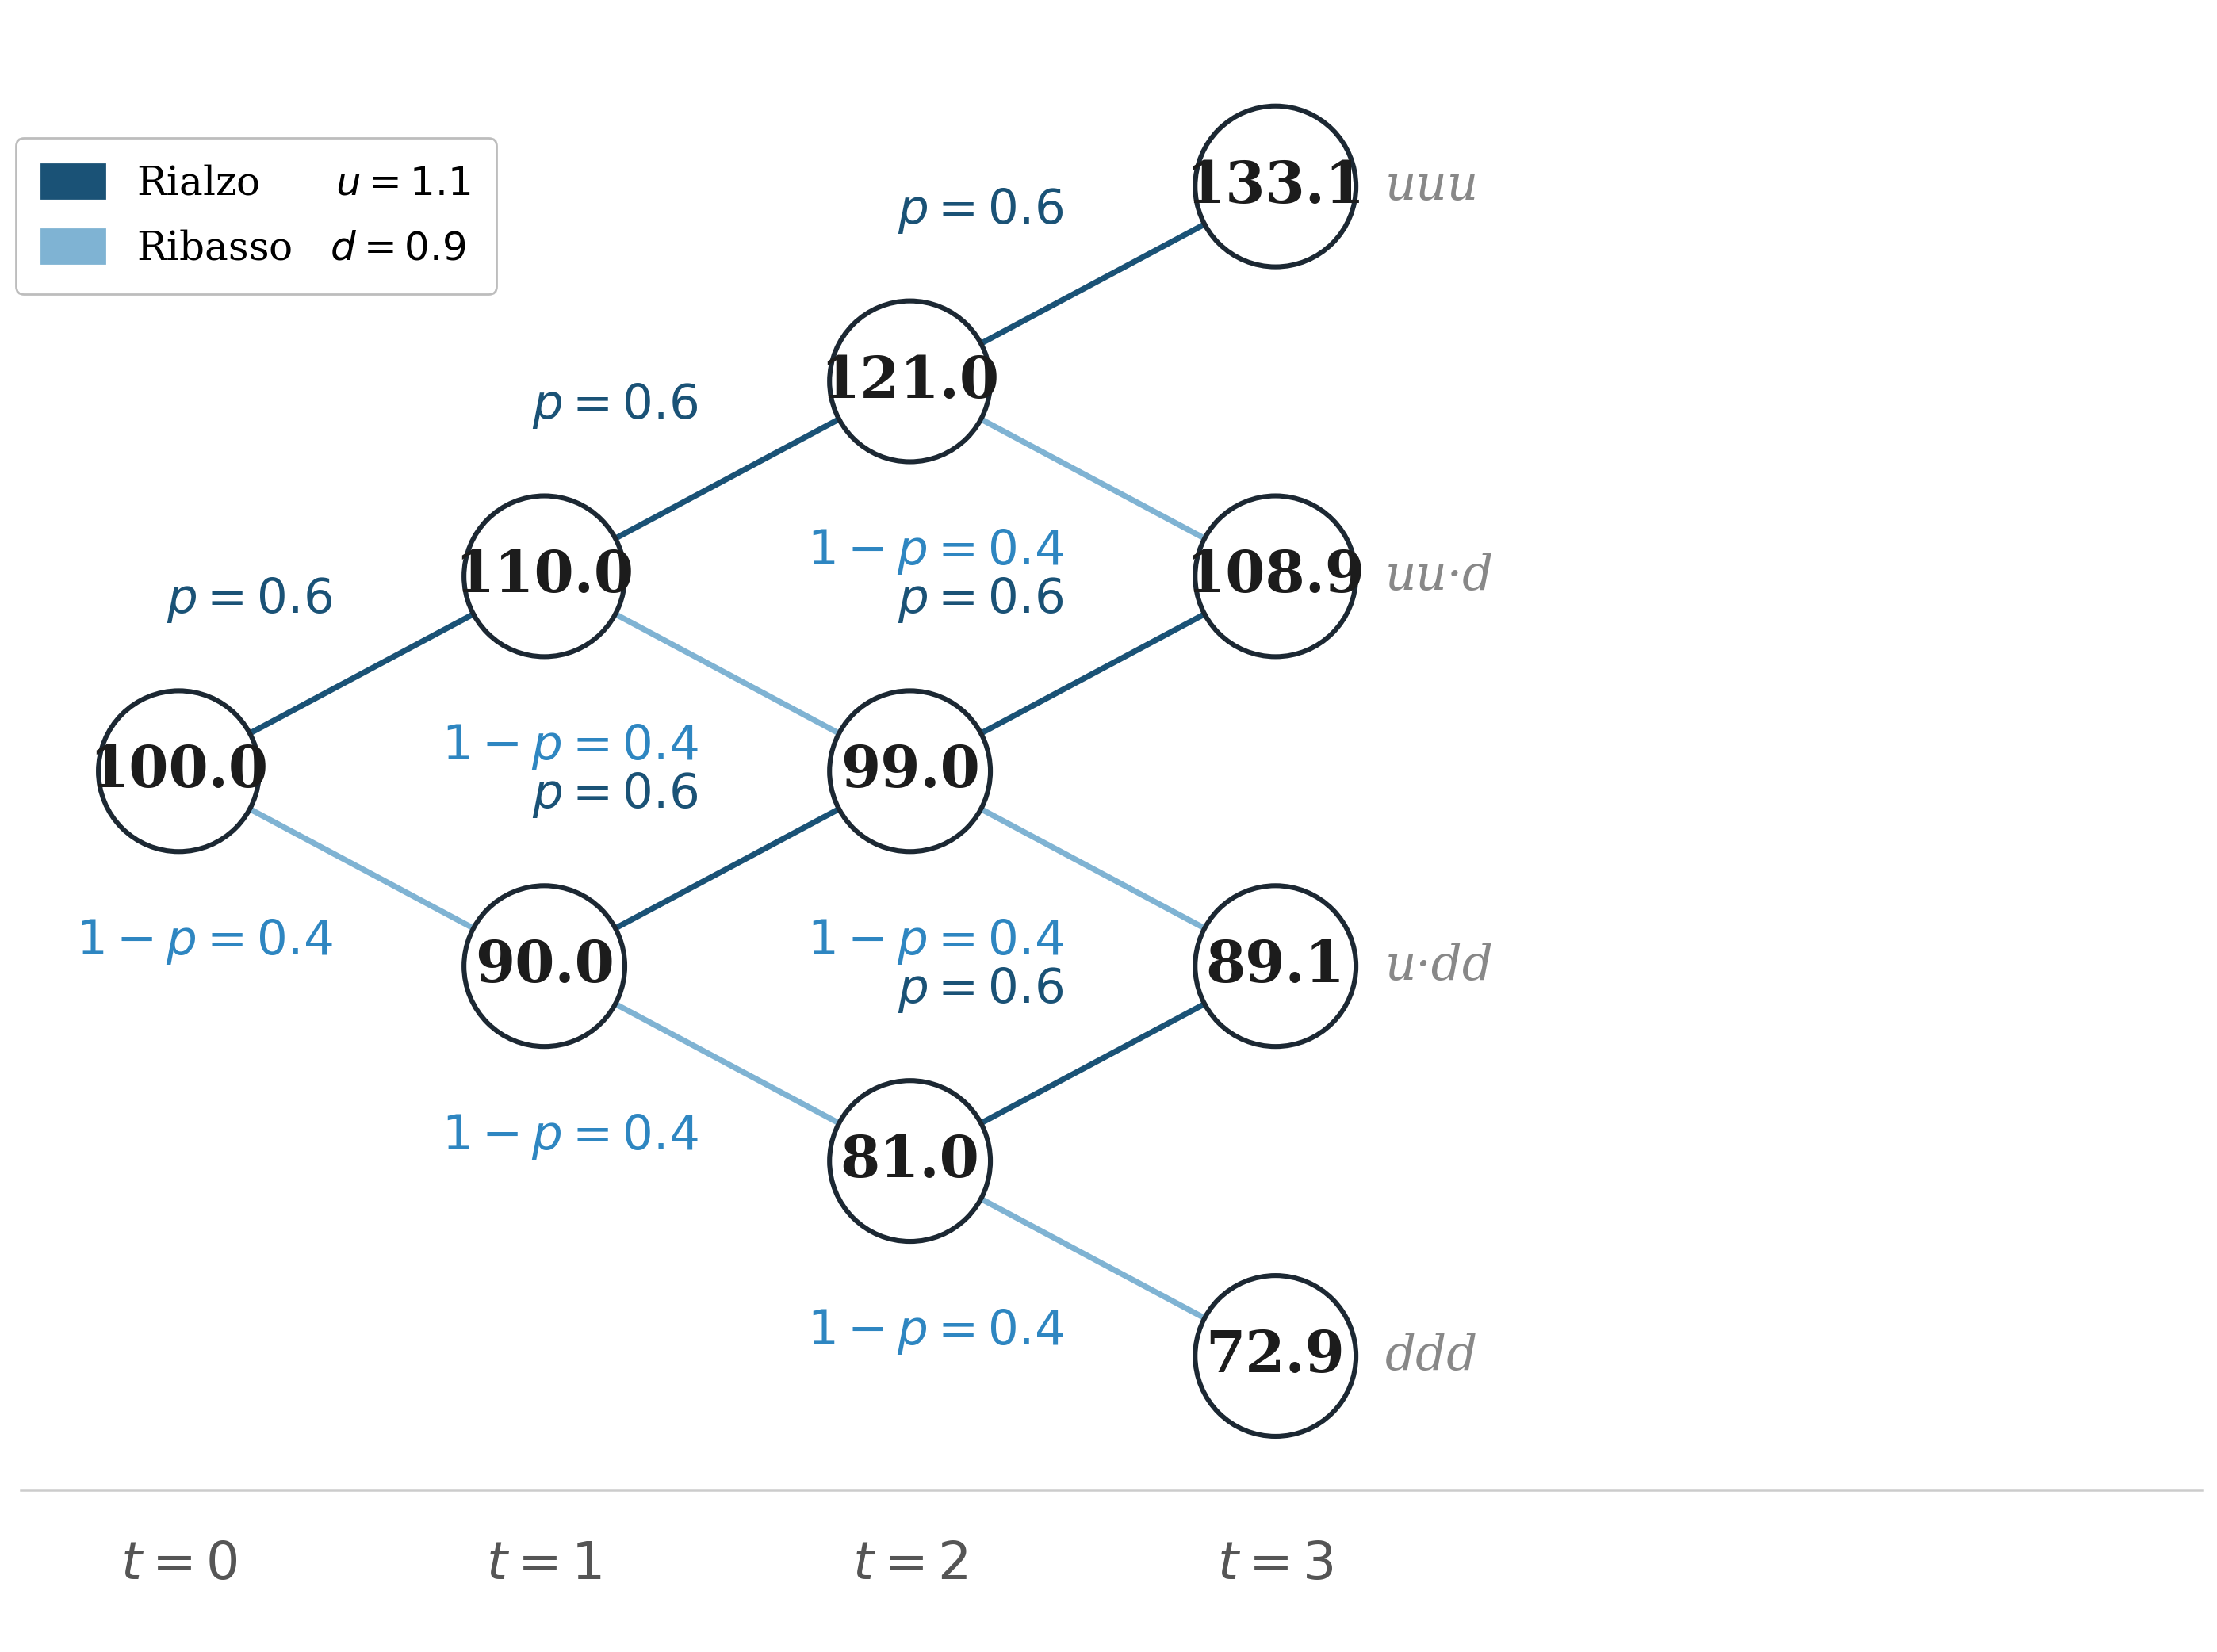
\includegraphics[width=\linewidth]{../graphics/Cap05_Figura_5_1}
\end{column}
 
\begin{column}{0.35\textwidth}
L'albero \textbf{ricombina}: al tempo $t$ vi sono $t+1$ nodi
di prezzo distinti, pur essendovi $2^t$ storie possibili.
\end{column}
 
\end{columns}
 
%TCIMACRO{\TeXButton{Transition: Box Out}{\transboxout}}%
%BeginExpansion
\transboxout
%EndExpansion
%TCIMACRO{\TeXButton{EndFrame}{\end{frame}}}%
%BeginExpansion
\end{frame}%
%EndExpansion

% --------------------------------------------------------
% Slide 28 -- Sigma-algebre e partizioni sull'albero
% --------------------------------------------------------

\subsection{Sigma-algebre e partizioni}

%TCIMACRO{\TeXButton{BeginFrame}{\begin{frame}}}%
%BeginExpansion
\begin{frame}%
%EndExpansion

\QTR{frametitle}{Sigma-algebre e partizioni sull'albero}

%TCIMACRO{\TeXButton{Transparency}{\setbeamercovered{transparent=20}}}%
%BeginExpansion
\setbeamercovered{transparent=20}%
%EndExpansion

Con $T=3$, $\Omega=\{uuu,uud,udu,udd,duu,dud,ddu,ddd\}$.

\medskip

{\footnotesize
\begin{center}
\begin{tabular}{|p{0.4cm}|p{2.6cm}|p{6.4cm}|}
\hline
$t$ & \textbf{Sigma-algebra} & \textbf{Partizione di $\Omega$}\\
\hline
$0$ & $\F_0=\{\emptyset,\Omega\}$ &
Unico blocco: \newline $\{uuu,uud,udu,udd,duu,dud,ddu,ddd\}$\\[4pt]
$1$ & $\F_1=\sigma(S_1)$ &
Due blocchi: \newline $A_u=\{uuu,uud,udu,udd\}$ e \newline
$A_d=\{duu,dud,ddu,ddd\}$\\[4pt]
$2$ & $\F_2=\sigma(S_1,S_2)$ &
Quattro blocchi: $A_{uu}=\{uuu,uud\}$,
$A_{ud}=\{udu,udd\}$,
$A_{du}=\{duu,dud\}$,
$A_{dd}=\{ddu,ddd\}$\\[4pt]
$3$ & $\F_3=\sigma(S_1,S_2,S_3)$ &
Otto blocchi: ogni esito elementare forma un blocco
da solo, ad esempio $\{uuu\}$, $\{uud\}$, \ldots,
$\{ddd\}$\\
\hline
\end{tabular}
\end{center}
}

\medskip

\begin{stepitemize}
\item Al crescere di $t$ la partizione si affina:
l'informazione disponibile aumenta.
\item Due traiettorie nello stesso blocco di $\F_t$
sono \textbf{indistinguibili} sulla base di quanto
osservato fino a $t$.
\end{stepitemize}

%TCIMACRO{\TeXButton{Transition: Box Out}{\transboxout}}%
%BeginExpansion
\transboxout
%EndExpansion
%TCIMACRO{\TeXButton{EndFrame}{\end{frame}}}%
%BeginExpansion
\end{frame}%
%EndExpansion

% --------------------------------------------------------
% Slide 29 -- Processo delle previsioni sull'albero
% --------------------------------------------------------

\subsection{Processo delle previsioni}

%TCIMACRO{\TeXButton{BeginFrame}{\begin{frame}}}%
%BeginExpansion
\begin{frame}%
%EndExpansion

\QTR{frametitle}{Il processo delle previsioni sull'albero}

%TCIMACRO{\TeXButton{Transparency}{\setbeamercovered{transparent=20}}}%
%BeginExpansion
\setbeamercovered{transparent=20}%
%EndExpansion

Definiamo $H_t=\E[S_3\mid\F_t]$: la previsione del prezzo
terminale aggiornata all'informazione disponibile al tempo $t$.

\medskip

\begin{stepitemize}

\item \textbf{Formula compatta}: poich\`{e} i fattori futuri
sono indipendenti da $\F_t$,
\[
H_t=\E[S_3\mid\F_t]=S_t\cdot m^{3-t}.
\]
La previsione \`{e} il prezzo corrente capitalizzato al
rendimento medio $m$ per i periodi residui.

\item \textbf{Valori nei nodi} ($S_0=100$, $m=1.02$):
\begin{center}
{\small
\begin{tabular}{cl}
\hline
$t$ & Valori di $H_t$ nei nodi\\
\hline
$0$ & $106.12$\\
$1$ & $114.44$ (nodo $u$), $\quad 93.64$ (nodo $d$)\\
$2$ & $123.42$ ($uu$), $100.98$ ($ud$), $82.62$ ($dd$)\\
$3$ & $133.10$, $108.90$, $89.10$, $72.90$\\
\hline
\end{tabular}
}
\end{center}

\item \textbf{Verifica al nodo $u$, $t=1\to 2$}:
\[
\E[H_2\mid A_u]=0.6\cdot123.42+0.4\cdot100.98=114.44=H_1(A_u).
\]

\end{stepitemize}

%TCIMACRO{\TeXButton{Transition: Box Out}{\transboxout}}%
%BeginExpansion
\transboxout
%EndExpansion
%TCIMACRO{\TeXButton{EndFrame}{\end{frame}}}%
%BeginExpansion
\end{frame}%
%EndExpansion

% --------------------------------------------------------
% Slide 30 -- Martingala di Doob e prezzi
% --------------------------------------------------------

\subsection{Martingale sul binomiale}

%TCIMACRO{\TeXButton{BeginFrame}{\begin{frame}}}%
%BeginExpansion
\begin{frame}%
%EndExpansion

\QTR{frametitle}{Martingala di Doob e processo dei prezzi}

%TCIMACRO{\TeXButton{Transparency}{\setbeamercovered{transparent=20}}}%
%BeginExpansion
\setbeamercovered{transparent=20}%
%EndExpansion

\begin{stepitemize}

\item \textbf{$\{H_t\}$ \`{e} sempre una martingala.}
Per la propriet\`{a} della torre:
\[
\E[H_t\mid\F_s]=\E\bigl[\E[S_3\mid\F_t]\bigm|\F_s\bigr]
=\E[S_3\mid\F_s]=H_s.
\]
Le revisioni della previsione sono shock imprevedibili:
$\E[H_{t+1}-H_t\mid\F_t]=0$.

\item \textbf{$\{S_t\}$ \`{e} una martingala solo se $m=1$.}
\[
\E[S_{t+1}\mid\F_t]=S_t\cdot m.
\]
Con $m=1.02>1$: $\E[S_{t+1}\mid\F_t]>S_t$ --- il processo
dei prezzi \`{e} una \textbf{submartingala}.

\item \textbf{Attenzione}: non confondere il processo delle
previsioni $\{H_t\}$ con il processo dei prezzi $\{S_t\}$.
Il primo \`{e} sempre una martingala. Il secondo lo \`{e}
solo se il rendimento medio \`{e} unitario ($m=1$), condizione
alla base della valutazione risk-neutral.

\end{stepitemize}

%TCIMACRO{\TeXButton{Transition: Box Out}{\transboxout}}%
%BeginExpansion
\transboxout
%EndExpansion
%TCIMACRO{\TeXButton{EndFrame}{\end{frame}}}%
%BeginExpansion
\end{frame}%
%EndExpansion



% --------------------------------------------------------
% Slide 32 -- Sintesi del ruolo del binomiale
% --------------------------------------------------------

\subsection{Sintesi}

%TCIMACRO{\TeXButton{BeginFrame}{\begin{frame}}}%
%BeginExpansion
\begin{frame}%
%EndExpansion

\QTR{frametitle}{Il binomiale come palestra: sintesi}

%TCIMACRO{\TeXButton{Transparency}{\setbeamercovered{transparent=20}}}%
%BeginExpansion
\setbeamercovered{transparent=20}%
%EndExpansion

Il modello binomiale ha illustrato \textbf{concretamente}
ogni concetto generale della lezione:

\medskip

\begin{itemize}

\item \textbf{Processo}: $\{S_t\}$ con momenti $\mu(t)=S_0m^t$
e varianza crescente.

\item \textbf{Filtrazione}: la catena
$\F_0\subseteq\F_1\subseteq\F_2\subseteq\F_3$
come affinamento progressivo delle partizioni di $\Omega$.

\item \textbf{Adattato}: $S_t$ \`{e} $\F_t$-misurabile;
$S_{t+1}$ \`{e} anticipativo rispetto a $\F_t$.

\item \textbf{Martingala di Doob}: $H_t=S_t\,m^{3-t}$,
sempre martingala per la propriet\`{a} della torre.

\item \textbf{Submartingala}: $\{S_t\}$ con $m>1$; martingala
solo se $m=1$ (misura risk-neutral).

\item \textbf{Scenari e ricombinazione}: struttura ad albero
con crescita lineare dei nodi.

\end{itemize}

%TCIMACRO{\TeXButton{Transition: Box Out}{\transboxout}}%
%BeginExpansion
\transboxout
%EndExpansion
%TCIMACRO{\TeXButton{EndFrame}{\end{frame}}}%
%BeginExpansion
\end{frame}%
%EndExpansion

% ============================================================
% Slides_Lez_05_Gruppo_08_Esercizi.tex
% GRUPPO 8 -- Esercizi in aula
% Slide 34-37 (la numerazione esatta dipende dal totale
% effettivo del Gruppo 7 dopo le modifiche manuali)
% Tempo parziale: 12 minuti | Tempo cumulato: 130 minuti
% ============================================================

\section{Esercizi in aula}

% --------------------------------------------------------
% Slide -- Esercizio 1: calcolo
% --------------------------------------------------------

\subsection{Esercizio 1: calcolo}

%TCIMACRO{\TeXButton{BeginFrame}{\begin{frame}}}%
%BeginExpansion
\begin{frame}%
%EndExpansion

\QTR{frametitle}{Esercizio 1: albero binomiale a due periodi}

%TCIMACRO{\TeXButton{Transparency}{\setbeamercovered{transparent=20}}}%
%BeginExpansion
\setbeamercovered{transparent=20}%
%EndExpansion

\begin{block}{Dati}
Un'azione vale oggi $S_0=80$. A ogni periodo il prezzo sale
del $25\%$ ($u=1.25$, probabilit\`{a} $p=0.5$) oppure scende
del $20\%$ ($d=0.8$, probabilit\`{a} $1-p=0.5$). Orizzonte
$T=2$.
\end{block}

\medskip

\begin{stepenumerate}
\item Costruire l'albero dei prezzi ed elencare gli scenari
con le rispettive probabilit\`{a}.
\item Calcolare $\E[S_2]$, sia sommando sugli scenari sia con
la formula $S_0\,m^2$.
\item Calcolare $\E[S_2\mid\F_1]$ nei due nodi al tempo $1$
e verificare la propriet\`{a} della torre.
\end{stepenumerate}

\medskip

\begin{center}
{\small Tempo: 6 minuti.}
\end{center}

%TCIMACRO{\TeXButton{Transition: Box Out}{\transboxout}}%
%BeginExpansion
\transboxout
%EndExpansion
%TCIMACRO{\TeXButton{EndFrame}{\end{frame}}}%
%BeginExpansion
\end{frame}%
%EndExpansion

% --------------------------------------------------------
% Slide -- Esercizio 1: soluzione
% --------------------------------------------------------

%TCIMACRO{\TeXButton{BeginFrame}{\begin{frame}}}%
%BeginExpansion
\begin{frame}%
%EndExpansion

\QTR{frametitle}{Esercizio 1: soluzione}

%TCIMACRO{\TeXButton{Transparency}{\setbeamercovered{transparent=20}}}%
%BeginExpansion
\setbeamercovered{transparent=20}%
%EndExpansion

\begin{stepitemize}

\item $m=pu+(1-p)d=0.5\cdot1.25+0.5\cdot0.8=1.025$.
\[
S_1^u=100,\quad S_1^d=64,\qquad
S_2^{uu}=125,\;\; S_2^{ud}=S_2^{du}=80,\;\; S_2^{dd}=51.2.
\]

\item $\E[S_2]=0.25\cdot125+0.5\cdot80+0.25\cdot51.2=84.05$.\\
Verifica: $S_0\,m^2=80\cdot1.025^2=84.05$.

\item Al nodo $u$: $\E[S_2\mid A_u]=0.5\cdot125+0.5\cdot80
=102.5=100\cdot1.025$.\\
Al nodo $d$: $\E[S_2\mid A_d]=0.5\cdot80+0.5\cdot51.2
=65.6=64\cdot1.025$.

\item Torre: $0.5\cdot102.5+0.5\cdot65.6=84.05=\E[S_2]$.
\checkmark

\end{stepitemize}

%TCIMACRO{\TeXButton{Transition: Box Out}{\transboxout}}%
%BeginExpansion
\transboxout
%EndExpansion
%TCIMACRO{\TeXButton{EndFrame}{\end{frame}}}%
%BeginExpansion
\end{frame}%
%EndExpansion

% --------------------------------------------------------
% Slide -- Esercizio 2: interpretazione
% --------------------------------------------------------

\subsection{Esercizio 2: interpretazione}

%TCIMACRO{\TeXButton{BeginFrame}{\begin{frame}}}%
%BeginExpansion
\begin{frame}%
%EndExpansion

\QTR{frametitle}{Esercizio 2: interpretazione finanziaria}

%TCIMACRO{\TeXButton{Transparency}{\setbeamercovered{transparent=20}}}%
%BeginExpansion
\setbeamercovered{transparent=20}%
%EndExpansion

\begin{block}{Scenario}
Un desk di trading accumula profitti giornalieri $Z_k$ i.i.d.,
con $\E[Z_k]=\nu>0$. Sia $X_t=\sum_{k=1}^t Z_k$ il profitto
cumulato.
\end{block}

\medskip

\begin{stepenumerate}
\item Il processo $\{X_t\}$ \`{e} una martingala, una
submartingala o una supermartingala rispetto alla propria
filtrazione naturale? Motivare.
\item Cosa cambia se $\nu=0$? E se $\nu<0$?
\item Interpretare finanziariamente i tre casi: cosa
rappresenta $\nu$ per un gestore che valuta la strategia?
\end{stepenumerate}

\medskip

\begin{center}
{\small Tempo: 6 minuti.}
\end{center}

%TCIMACRO{\TeXButton{Transition: Box Out}{\transboxout}}%
%BeginExpansion
\transboxout
%EndExpansion
%TCIMACRO{\TeXButton{EndFrame}{\end{frame}}}%
%BeginExpansion
\end{frame}%
%EndExpansion

% --------------------------------------------------------
% Slide -- Esercizio 2: soluzione
% --------------------------------------------------------

%TCIMACRO{\TeXButton{BeginFrame}{\begin{frame}}}%
%BeginExpansion
\begin{frame}%
%EndExpansion

\QTR{frametitle}{Esercizio 2: soluzione}

%TCIMACRO{\TeXButton{Transparency}{\setbeamercovered{transparent=20}}}%
%BeginExpansion
\setbeamercovered{transparent=20}%
%EndExpansion

\begin{stepitemize}

\item Per $s\leq t$: $\E[X_t\mid\F_s]=X_s+(t-s)\nu$. Con
$\nu>0$: $\E[X_t\mid\F_s]\geq X_s$ $\Rightarrow$
\textbf{submartingala}.

\item Se $\nu=0$: $\E[X_t\mid\F_s]=X_s$ $\Rightarrow$
\textbf{martingala} (gioco equo). Se $\nu<0$:
\textbf{supermartingala} (gioco sfavorevole).

\item \textbf{Interpretazione}: $\nu$ \`{e} l'\emph{alpha}
della strategia --- il rendimento atteso per periodo al netto
di ogni componente aleatoria. $\nu>0$ segnala un vantaggio
sistematico (la strategia batte un gioco equo in media);
$\nu=0$ segnala l'assenza di vantaggio; $\nu<0$ segnala
costi che superano il rendimento lordo.

\item Collegamento alla decomposizione di Doob--Meyer
(Sezione~5.5): $X_t=(X_t-t\nu)+t\nu$, dove $X_t-t\nu$ \`{e}
la componente di gioco equo e $t\nu$ la tendenza prevedibile.

\end{stepitemize}

%TCIMACRO{\TeXButton{Transition: Box Out}{\transboxout}}%
%BeginExpansion
\transboxout
%EndExpansion
%TCIMACRO{\TeXButton{EndFrame}{\end{frame}}}%
%BeginExpansion
\end{frame}%
%EndExpansion

\end{document}